\appendix

\section{Details of experiment setting}
\label{apdx:detail}
Our test machine is equipped with an Intel i9-7920X CPU and two GTX1080Ti GPU. The operating system is Ubuntu 16.04 LTS and uses the configuration of python3.5.2 + torch0.4.1 + gym0.10.8 + mujoco-py1.50.1.62 + mujoco150.

\section{Figures for training process}
\label{apdx:allfigure}
\begin{figure*}[htb]
   \centering
      \subfigure[$\alpha = 0$]{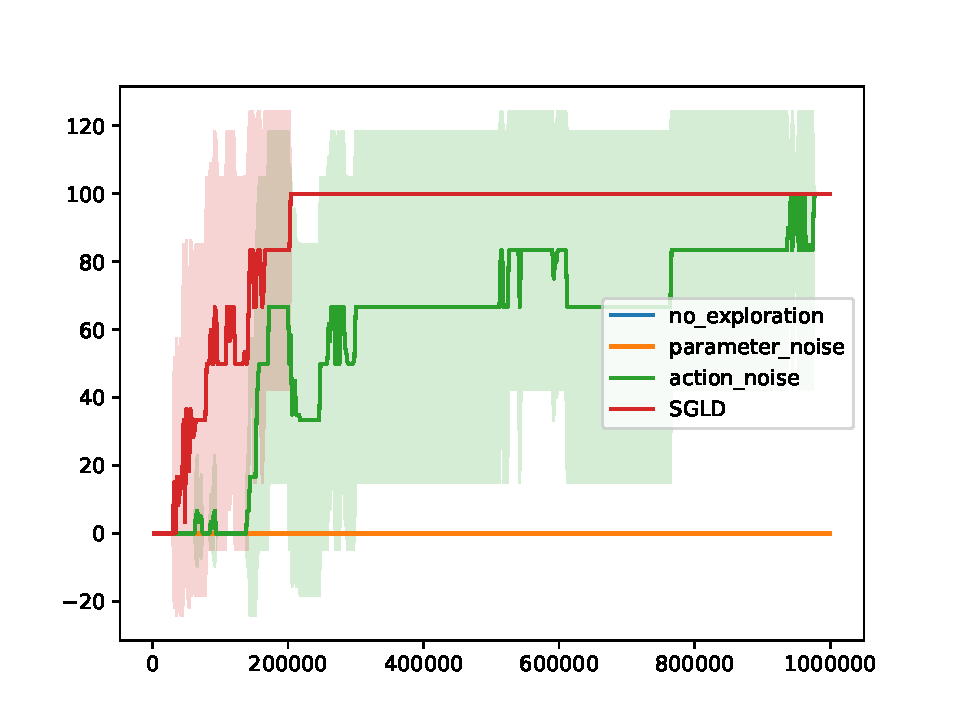
\includegraphics[width=150pt]{figs/MC0.pdf}}
      \subfigure[$\alpha = 0.1$]{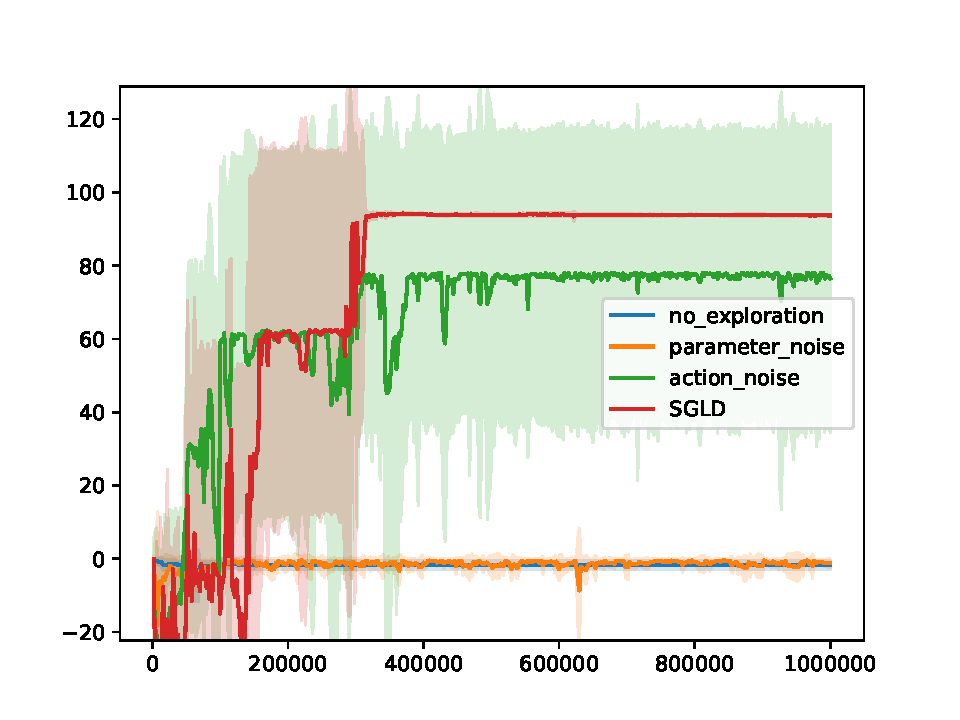
\includegraphics[width=150pt]{figs/MC.pdf}}
      \subfigure[$\alpha = 0.2$]{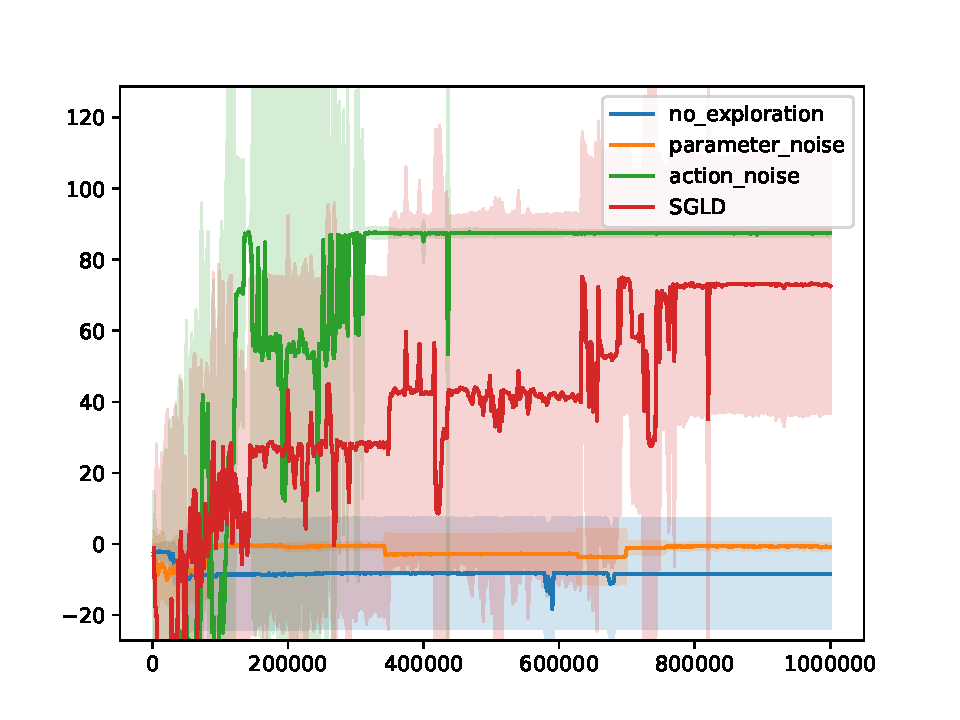
\includegraphics[width=150pt]{figs/MC0_2.pdf}}
      \subfigure[$\alpha = 0.5$]{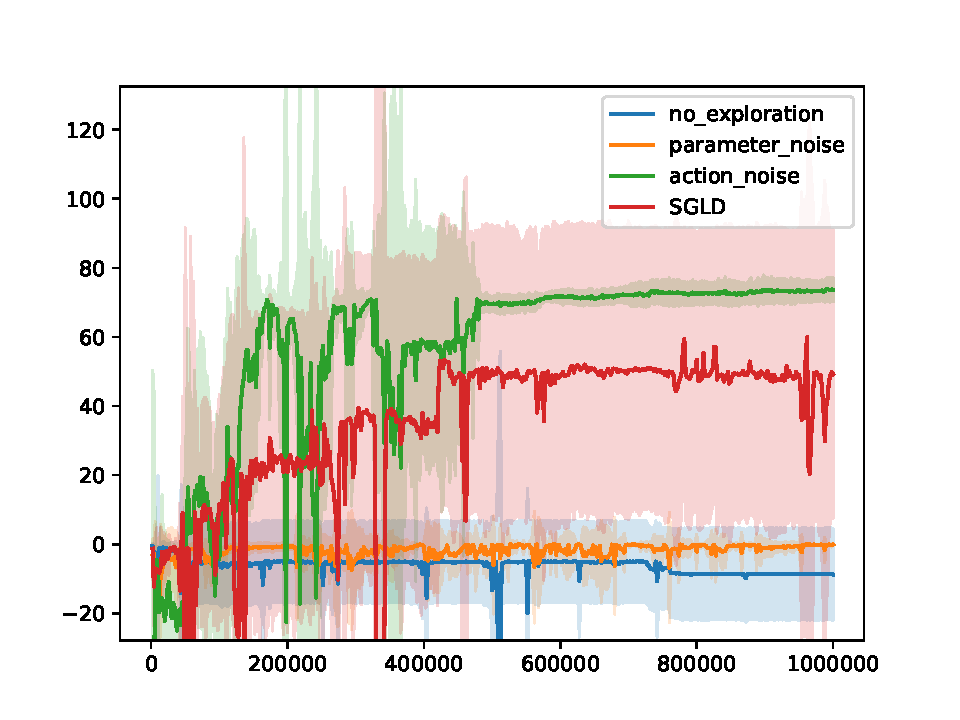
\includegraphics[width=150pt]{figs/MC0_5.pdf}}
      \subfigure[$\alpha = 1$]{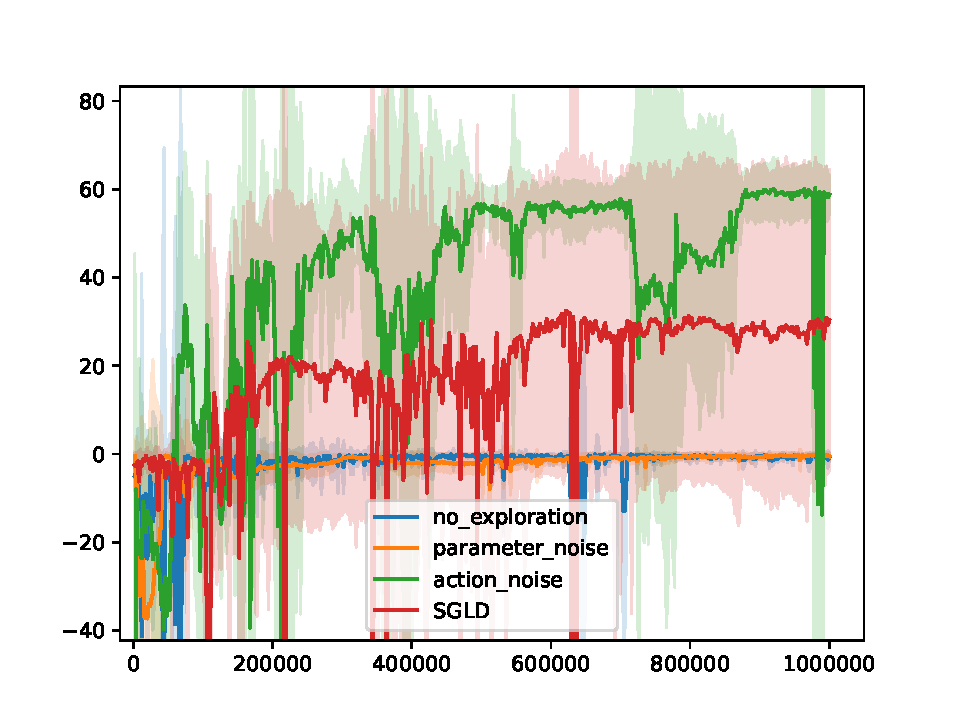
\includegraphics[width=150pt]{figs/MC1.pdf}}
   \label{fig:MCfigure}   
   \caption{MountainCar}
\end{figure*}
\begin{figure*}[htb]
   \centering
      \subfigure[$\alpha = 0$]{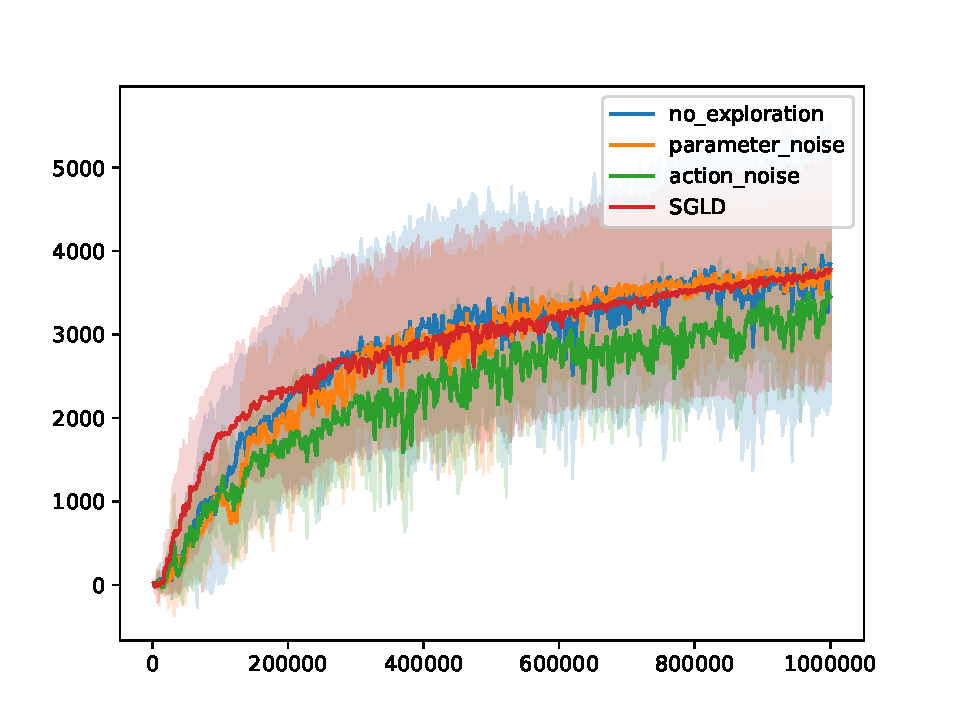
\includegraphics[width=150pt]{figs/HC0.pdf}}
      \subfigure[$\alpha = 0.1$]{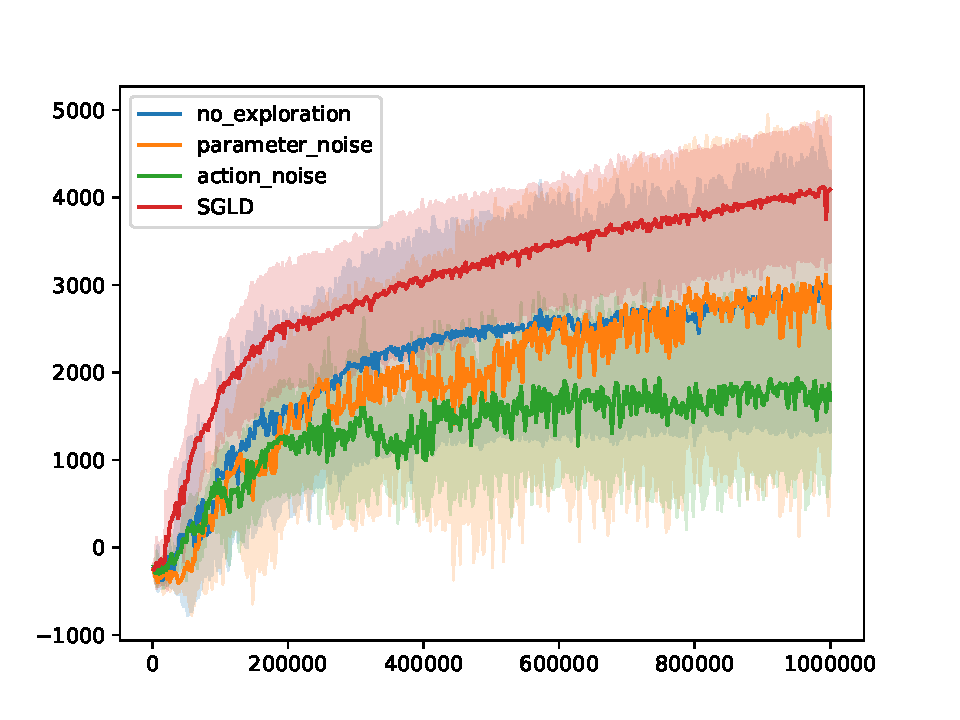
\includegraphics[width=150pt]{figs/HC.pdf}}
      \subfigure[$\alpha = 0.2$]{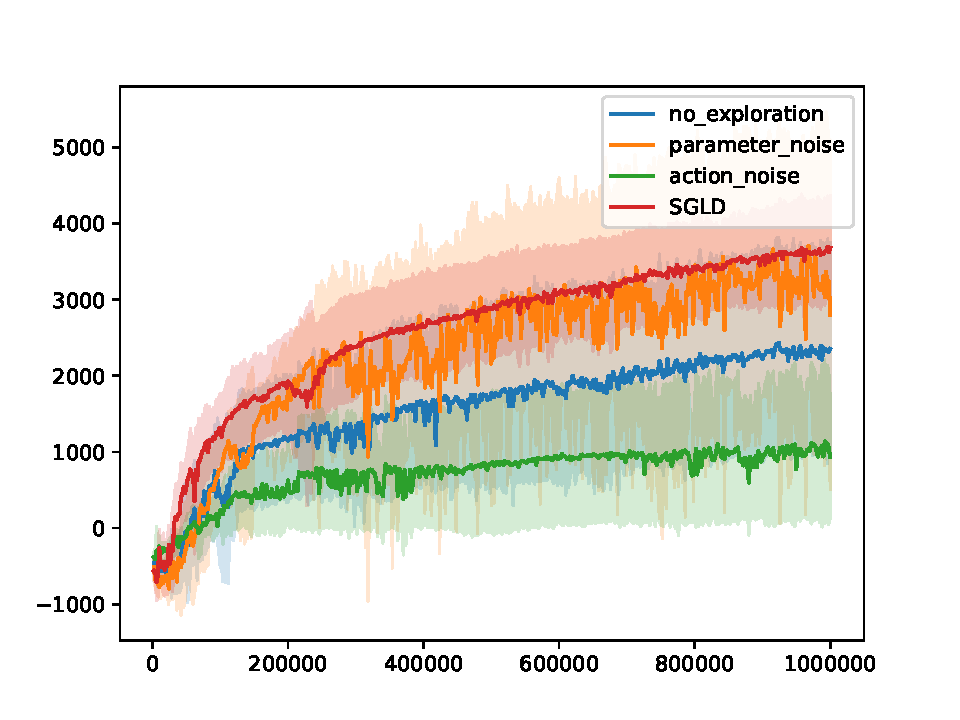
\includegraphics[width=150pt]{figs/HC0_2.pdf}}
      \subfigure[$\alpha = 0.5$]{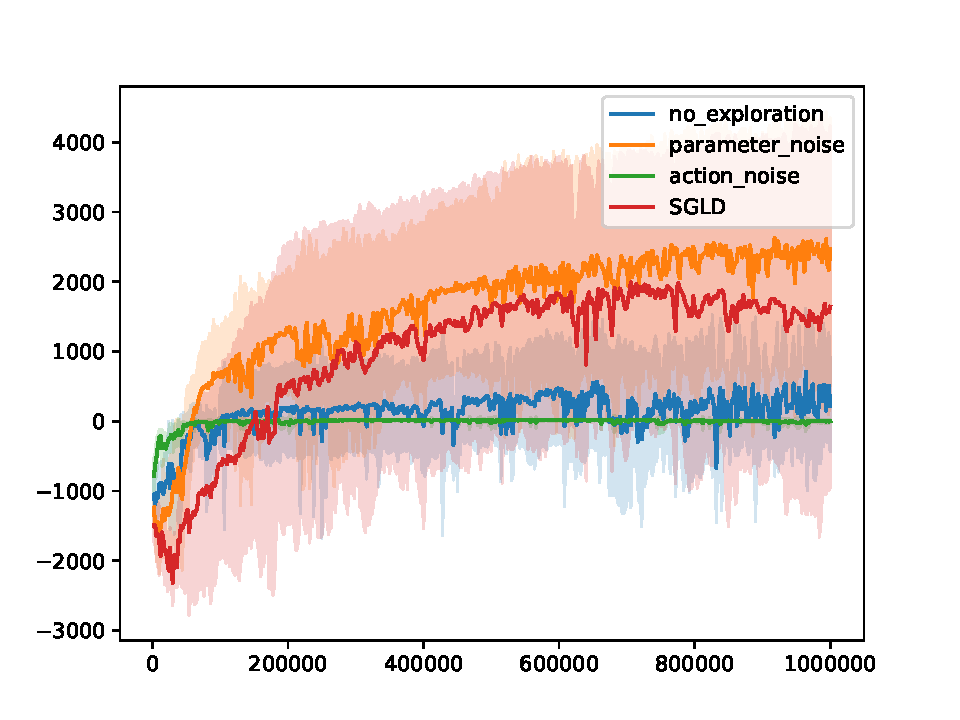
\includegraphics[width=150pt]{figs/HC0_5.pdf}}
      \subfigure[$\alpha = 1$]{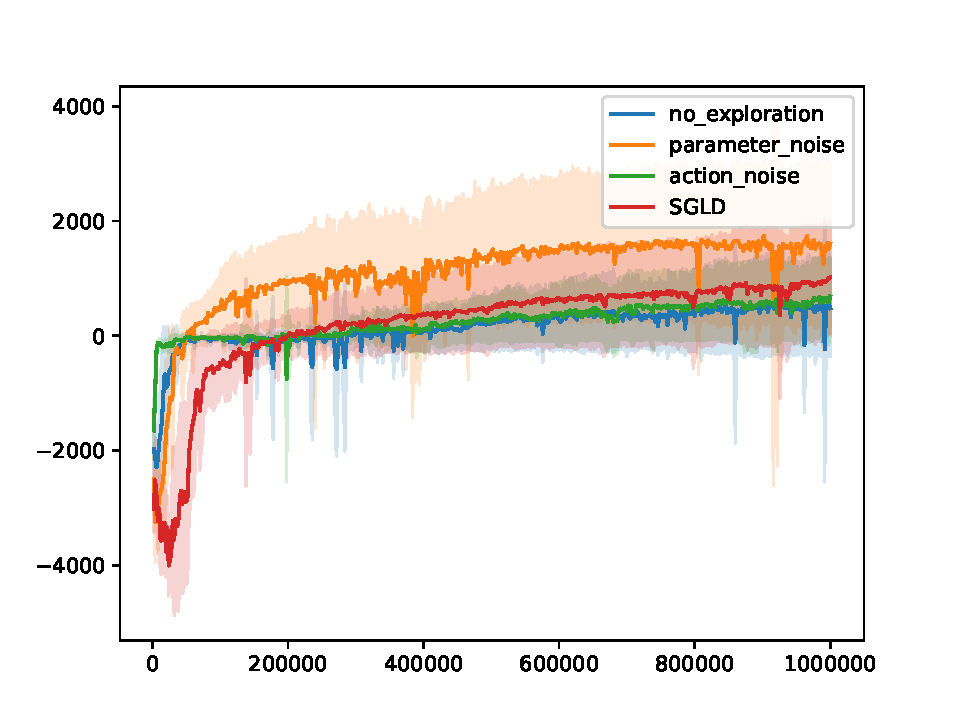
\includegraphics[width=150pt]{figs/HC1.pdf}}
   \label{fig:HCfigure}   
   \caption{HalfCheetah}
\end{figure*}
\begin{figure*}[htb]
   \centering
      \subfigure[$d = 1$]{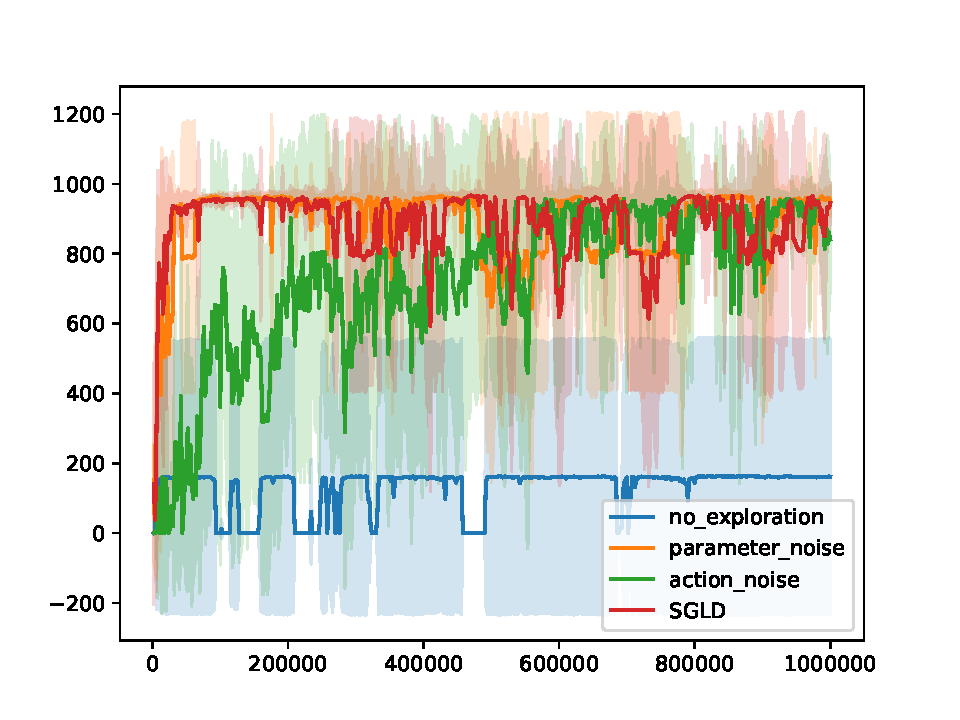
\includegraphics[width=150pt]{figs/SHC1.pdf}}
      \subfigure[$d = 2.5$]{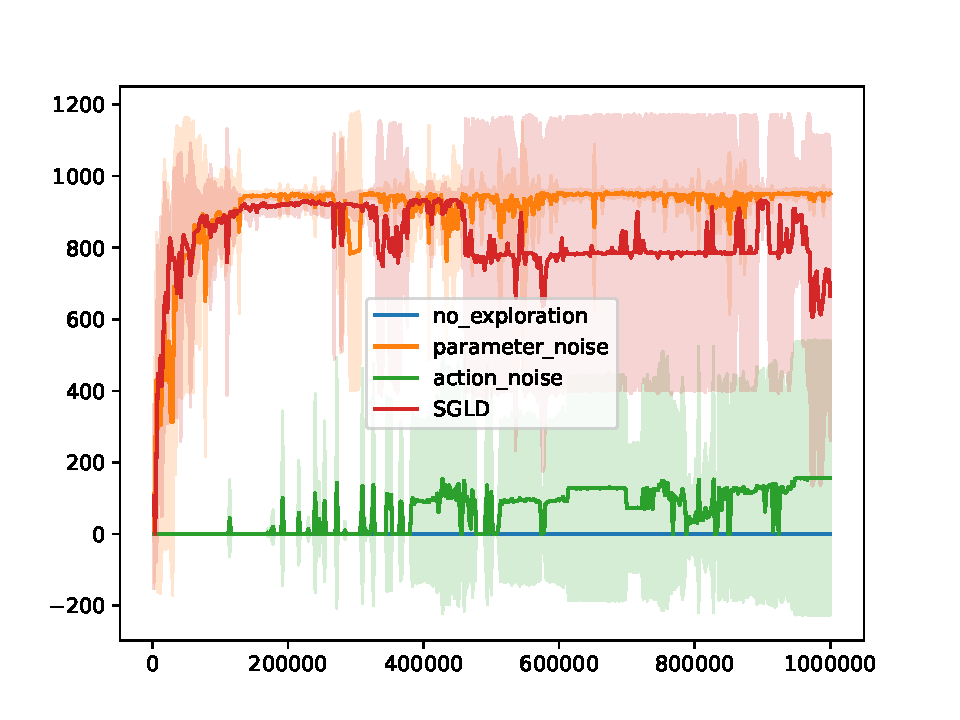
\includegraphics[width=150pt]{figs/SHC2_5.pdf}}
      \subfigure[$d = 5$]{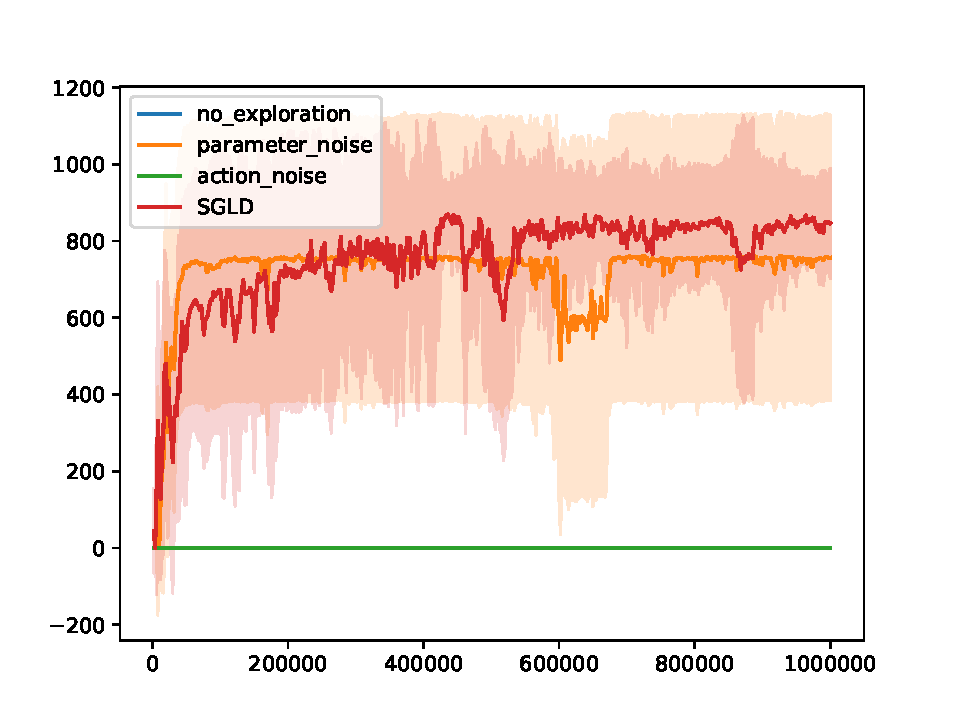
\includegraphics[width=150pt]{figs/SHC.pdf}}
      \subfigure[$d = 10$]{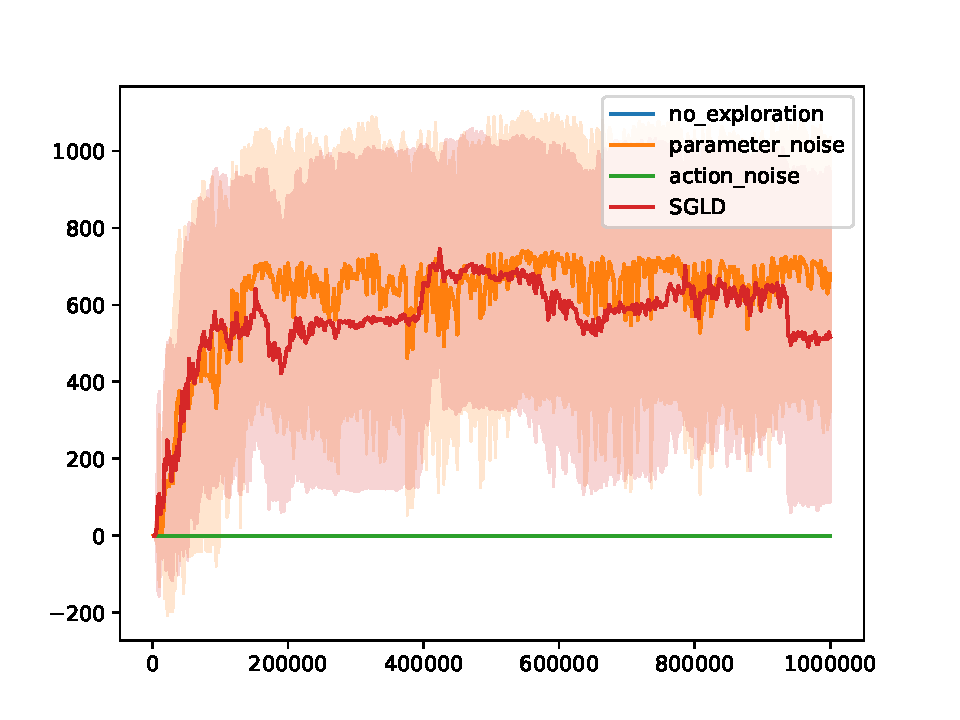
\includegraphics[width=150pt]{figs/SHC10.pdf}}
      \subfigure[$d = 20$]{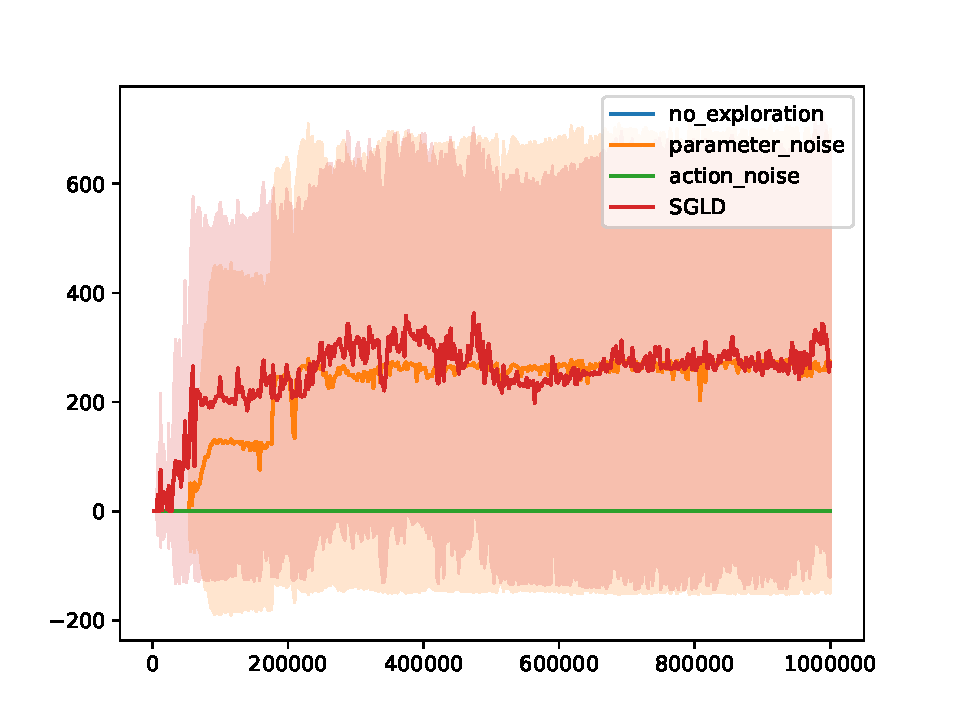
\includegraphics[width=150pt]{figs/SHC20.pdf}}
   \label{fig:SHCfigure}   
   \caption{Sparse HalfCheetah}
\end{figure*}
